\clearpage
\section{Risk Management}

\subsection{Risks}

\begin{table}[!ht]
    \makebox[\textwidth][c]{
        \begin{tabular}{ p{2cm} p{8.15cm} p{2cm} p{2cm}}
            \textbf{Risk Nr.} & \textbf{Description} & \textbf{Probability} & \textbf{Severity} \\ \hline \\                                                                                                                                                                           
            \textbf{R1} & Unfamiliar Technology (f.ex. Haskell Core) & 2 & 3 \\
            \textbf{R2} & Sickness & 1 & 2 \\
            \textbf{R3} & Goals set too high (too many or too complex features) & 2 & 1\\
            \textbf{R4} & Infeasibility of CLI Tool (not enough interactiveness) & 1 & 4\\
            \textbf{R5} & Infeasibility of GUI Tool (build too complex) & 2 & 1\\
            \textbf{R6} & Tool is too complicated (usability) & 1 & 3\\
            \textbf{R7} & Missing functionality of core stepper & 1 & 2\\
        \end{tabular}
    }
    \caption{Identified Risks in the Project}
    \label{tab:risks}
\end{table}

The identified risks can be visualized in the following risk matrix (Table \ref*{tab:risks}).

\begin{figure}[!ht]
    \centering
    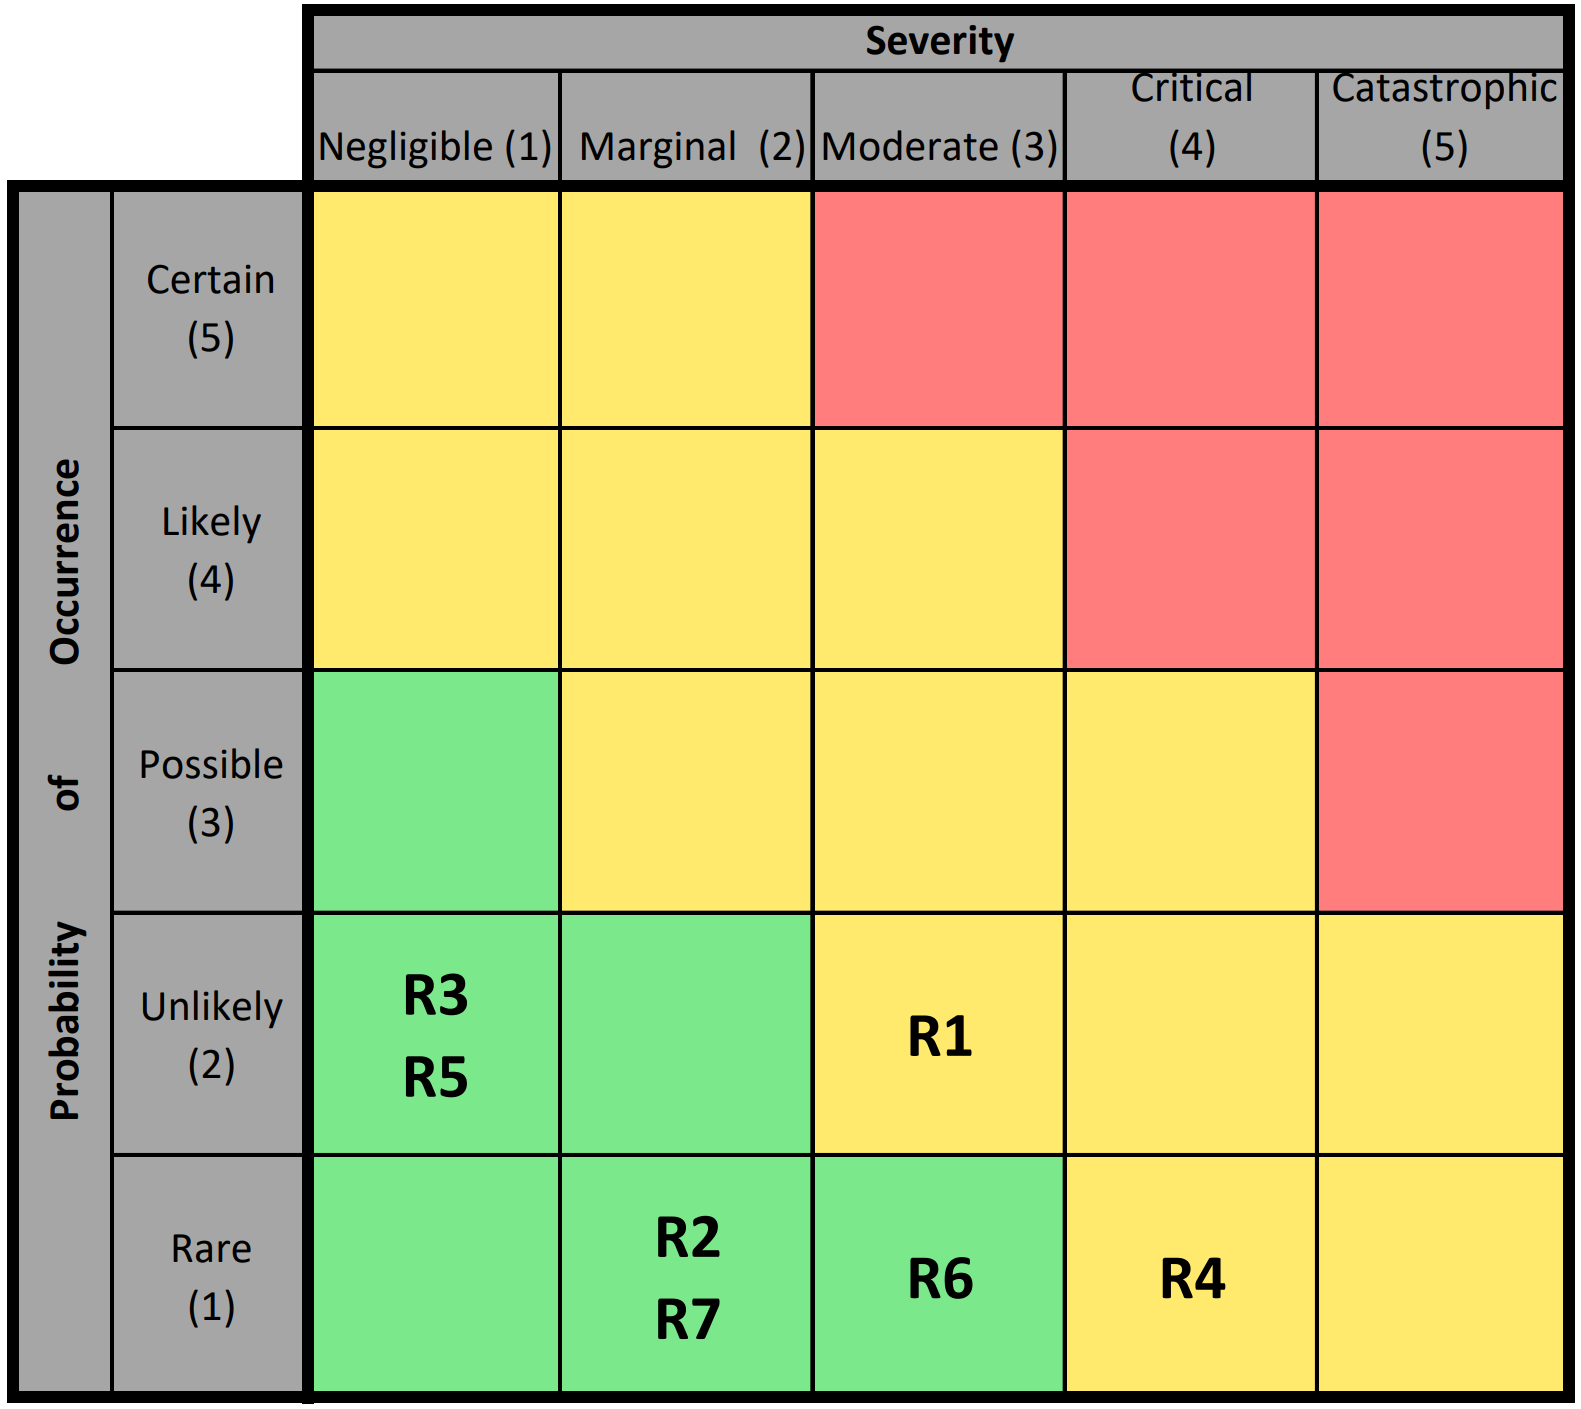
\includegraphics[width=0.6\textwidth]{resources/RiskMatrix.PNG}
    \caption{Risk Matrix}
    \label{fig:riskMatrix}
\end{figure}

\subsection{Mitigations}

In case one or more of the listed risks arise and turn into issues,
there are mitigations in place in order to reduce the severity of these issues.
These mitigations are shown in \ref*{tab:mitigations}.

\begin{table}[!ht]
    \makebox[\textwidth][c]{
        \begin{tabular}{ p{2cm} p{12.15cm}}
            \textbf{Risk Nr.} & \textbf{Mitigation} \\ \hline \\                                                                                                                                                                           
            \textbf{R1} & The people who worked on the stepper previously can be consulted in case there are any problems with existing software. \\
            \textbf{R2} & A time buffer at the end of the project is set in place, in case of sickness. \\
            \textbf{R3} & A time buffer at the end of the project is set in place, in case the estimates are too low. \\
            \textbf{R4} & A proof of concept is done at the start of the project. If it doesn't meet the requirements, a switch to a GUI could be done. \\
            \textbf{R5} & The GUI tool is not an essential feature and can thus be omitted. \\
            \textbf{R6} & Definition of an NFR that keeps the usage as simple as possible. \\
            \textbf{R7} & A time buffer at the end of the project is set in place, in case some functionality needs to be added in the core stepper. \\
        \end{tabular}
    }
    \caption{Mitigations for the identified risks.}
    \label{tab:mitigations}
\end{table}

\subsection{Arisen Issues}
During the project,
some of the risks that were identified during the planning of the project became issues.

\subsubsection*{R1}
It took me a while to get familiar with Core and to understand what was going on and how to understand the steps that are executed by the CoreStepper.
Luckily I could consider the developer of the CoreStepper for help and to understand what exactly was going on.
So while it took some time, it was not too much time that was spent on this.

\subsubsection*{R2}
While I got sick once,
that didn't affect the project too much,
as I was still able to put in work during that time.

\subsubsection*{Unforseen Risks}
Due to circumstances beyond my control,
an impactful incident in my private life kept me from working for about a week.
Thankfully, I was able to move the deadline of the project back by a week,
which mitigated this issue.
